\chapter[Resultados Obtenidos]{Resultados obtenidos para los proplyds ``clásicos''}
\label{chap:proplyds}
\thispagestyle{empty}
Probamos nuestro modelo descrito en los capítulos anteriores en una muestra de proplyds pertenecientes a la Nebulosa de Orión (ONC) que presentan un choque de proa. En la figura \ref{fig:proplyds-map} se muestran los proplyds que pertencen a nuestra muestra.

En todos los casos no fue posible medir el radio característico $R_{90}$ debido a que el brillo de la cáscara decae con el ángulo polar $\theta$ y no es detectable para ángulos del orden de $60^\circ$. Sin embargo, a continuación mostraremos la metodología para obtener la inclinación más probable de cada choque, así como los
parámetros del modelo de cada uno de éstos que nos indican su forma intrínseca.

\begin{figure*}
    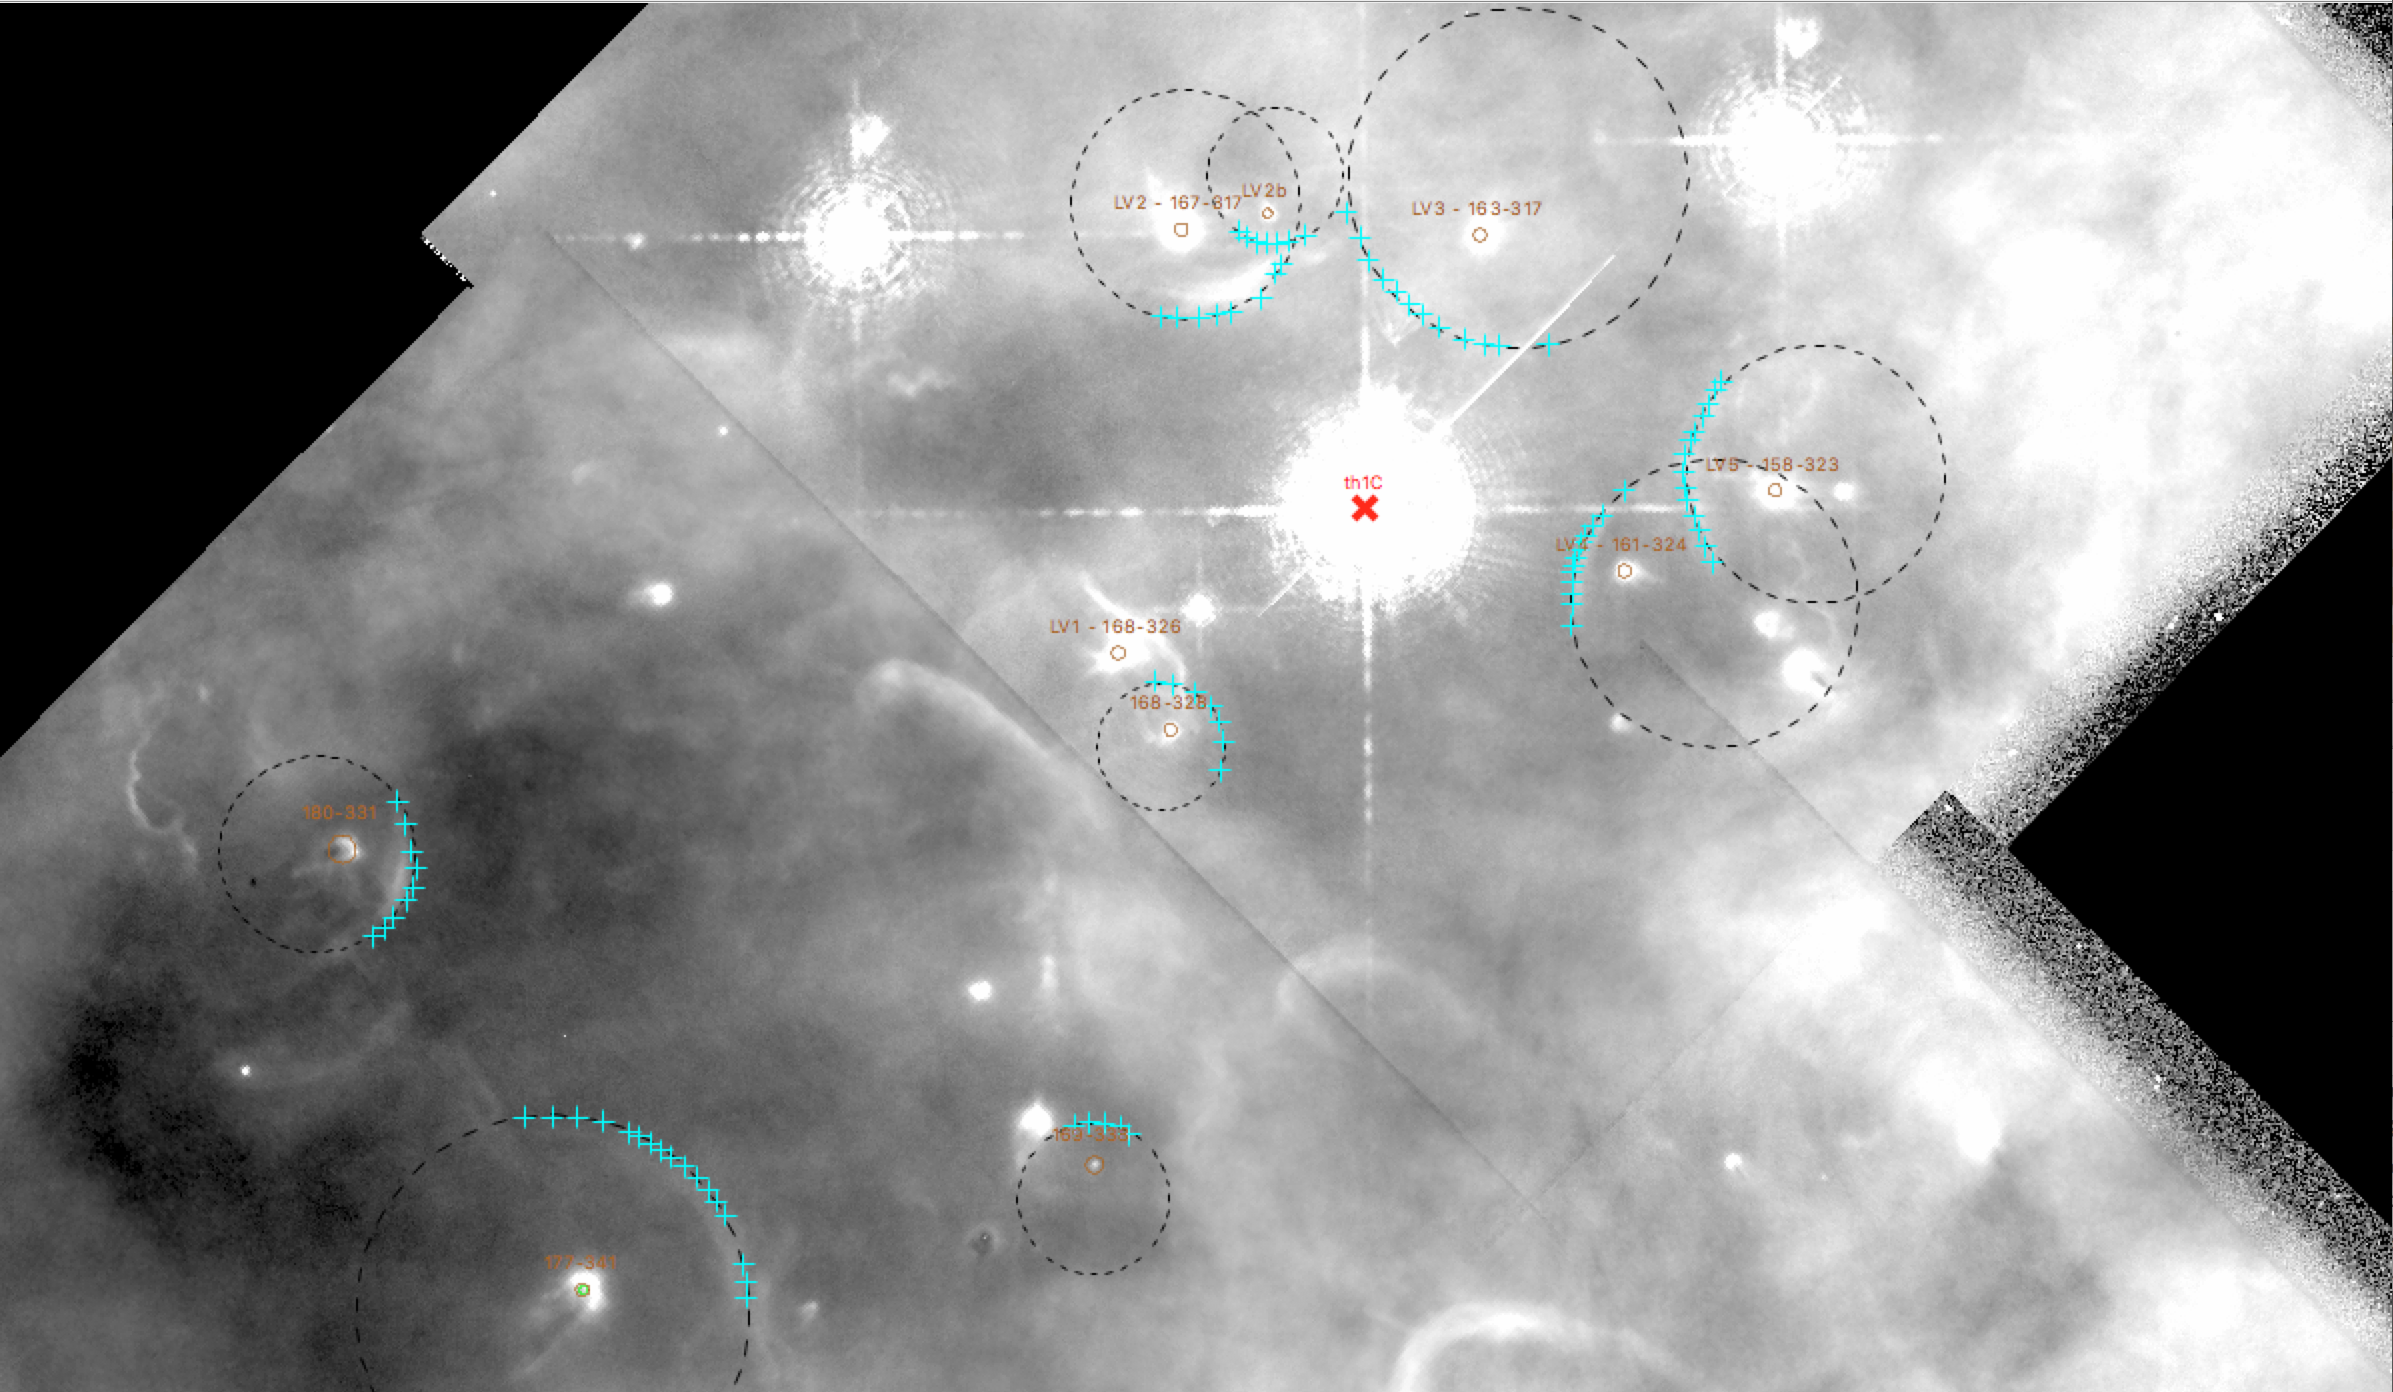
\includegraphics[width=\linewidth]{./Figures/LV-full-field-annotated}
    \caption{Imagen de la parte central de la Nebulosa de Orión donde se ubican los proplyds de nuestra muestra. Las cruces color cyan corresponden a las mediciones de la forma aparente para cada choque de proa. Los círculos amarillos marcan la posición de cada proplyd y la ``x'' roja corresponde a la posición de la estrella ionizante \thC{}. Los círculos negros ilustran de manera esquemática el radio de curvatura de cada choque.}
    \label{fig:proplyds-map}
\end{figure*}

\section{Metodología para la medición de la forma aparente.}
\label{sec:methodology}
Se utilizaron imágenes en el filtro de [\Ion{O}{III}] de la cámara WPC2 del Telescopio Espacial Hubble (HST). Se utilizaron las herramientas del programa DS9 para análisis de imágenes astronómicas para trazar la posición de \thC{} y de cada uno de los proplyds de la muestra. La posición y la forma de los choques de proa fue
trazada con una serie de marcas a lo largo del choque. Las coordenadas de las marcas fueron guardadas en un archivo y luego procesadas para tener las coordenadas del choque en el sistema de referencia del proplyd (Figura \ref{fig:proplyds-map}). El radio de curvatura aparente se obtiene haciendo un ajuste de mínimos cuadrados de la forma de un círculo de las mediciones obtenidas. $R_0$ se obtiene como la distancia mínima entre el proplyd y el ajuste circular dentro del rango de las coordenadas de las mediciones. 

\subsection{Medición de incertidumbres}

Para saber qué tan confiables son las coordenadas de las mediciones, se realizó el procedimiento siguiente: Del total de mediciones realizadas para cada proplyd, se crearon varias sub-muestras donde se utilizamos aproximadamente las dos terceras partes de las mediciones, pero dejando un mínimo de cuatro puntos, y se procedió a calcular los radios característicos para cada submuestra, y comprobar qué tanto se desvían estas mediciones de la original. En la figura \ref{fig:char-radii-obs} se muestran ejemplos de dichas sub-muestras para algunos proplyds.


\begin{figure*}
  \setkeys{Gin}{width=0.33\linewidth}%, trim=10 30 55 62.5}
\begin{tabular}{@{}c@{}c@{}c@{}}
 
Todos los puntos & Primera sub-muestra & Segunda sub-muestra \\ 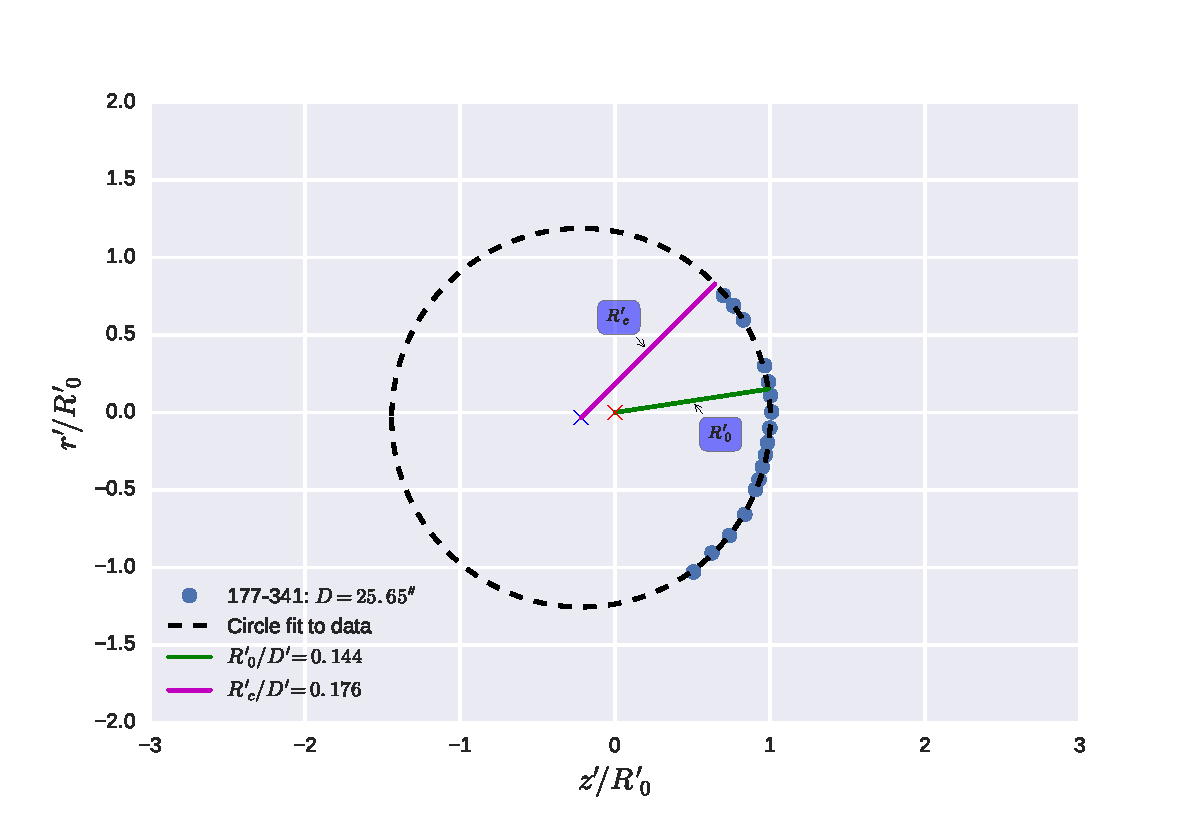
\includegraphics[clip]{./Figures/LV-bowshocks-xyfancy-positionswill-177-341} & 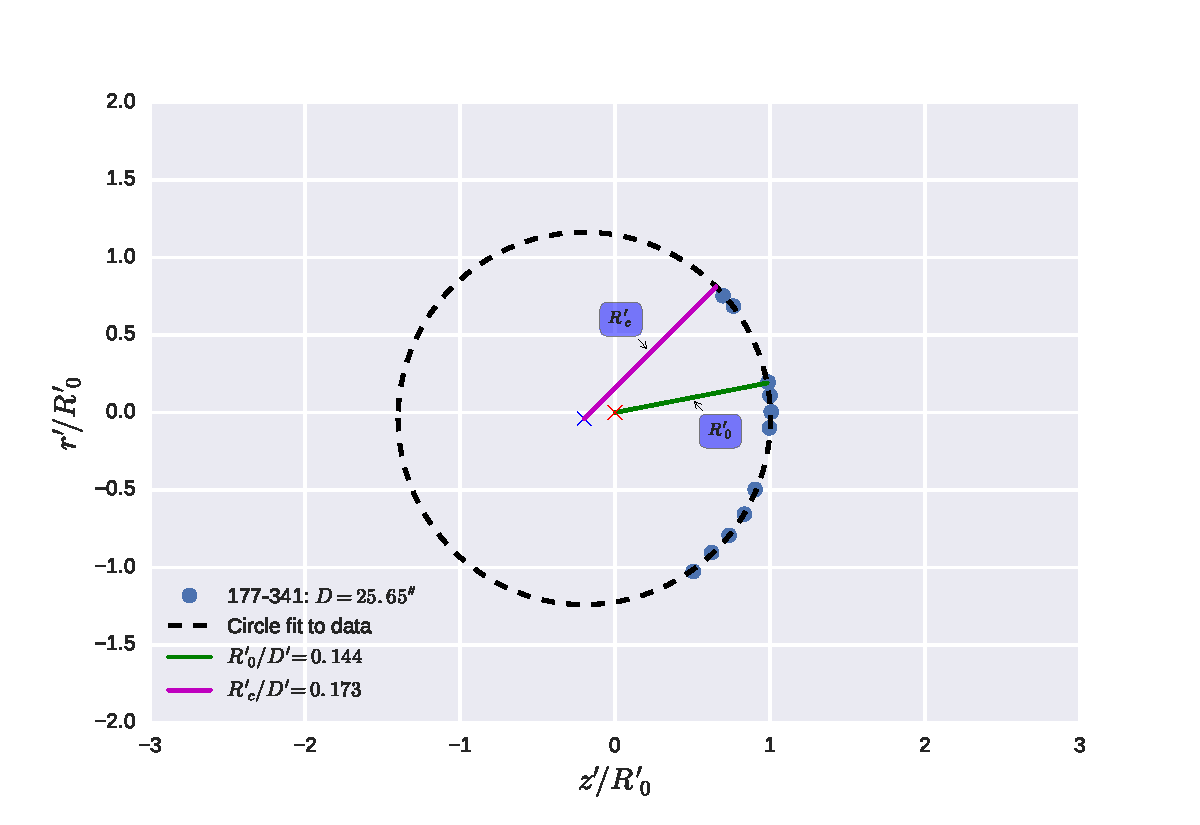
\includegraphics[clip]{./Figures/LV-bowshocks-xyfancy-positionssamp00-177-341} &
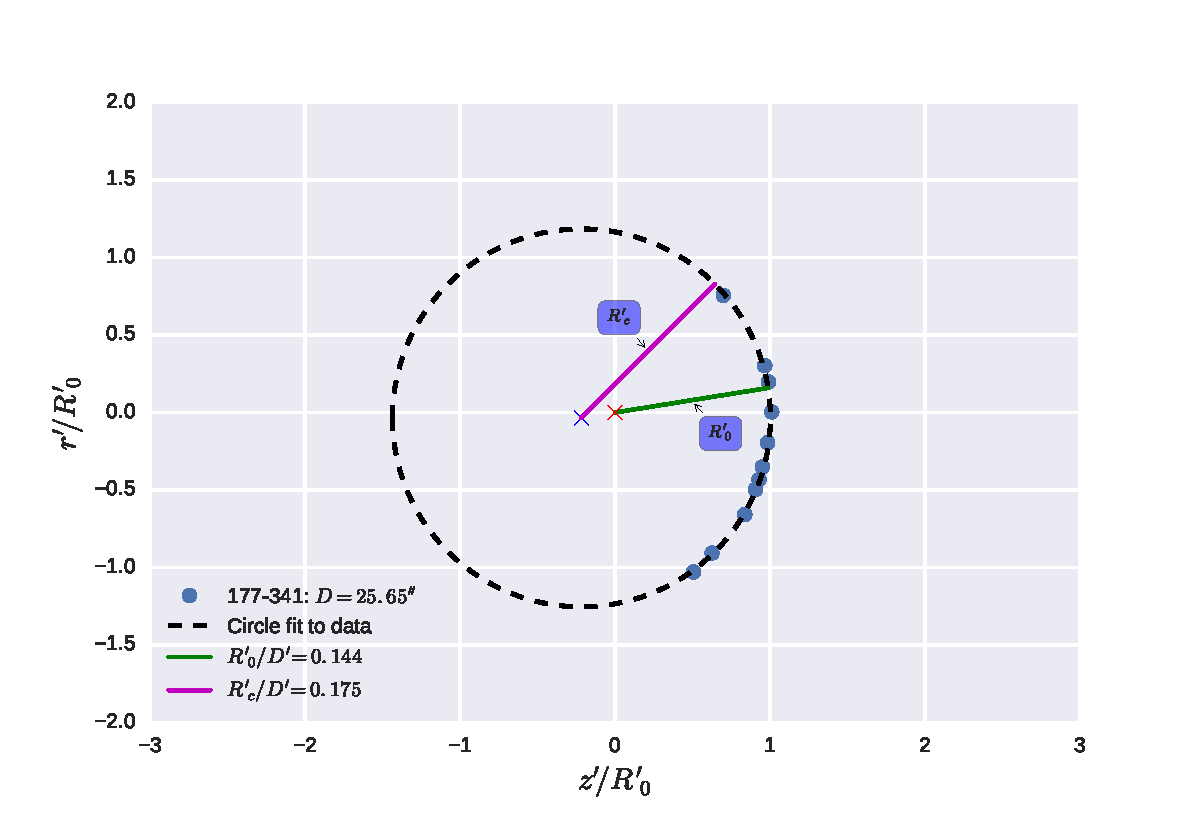
\includegraphics[clip]{./Figures/LV-bowshocks-xyfancy-positionssamp01-177-341} \\
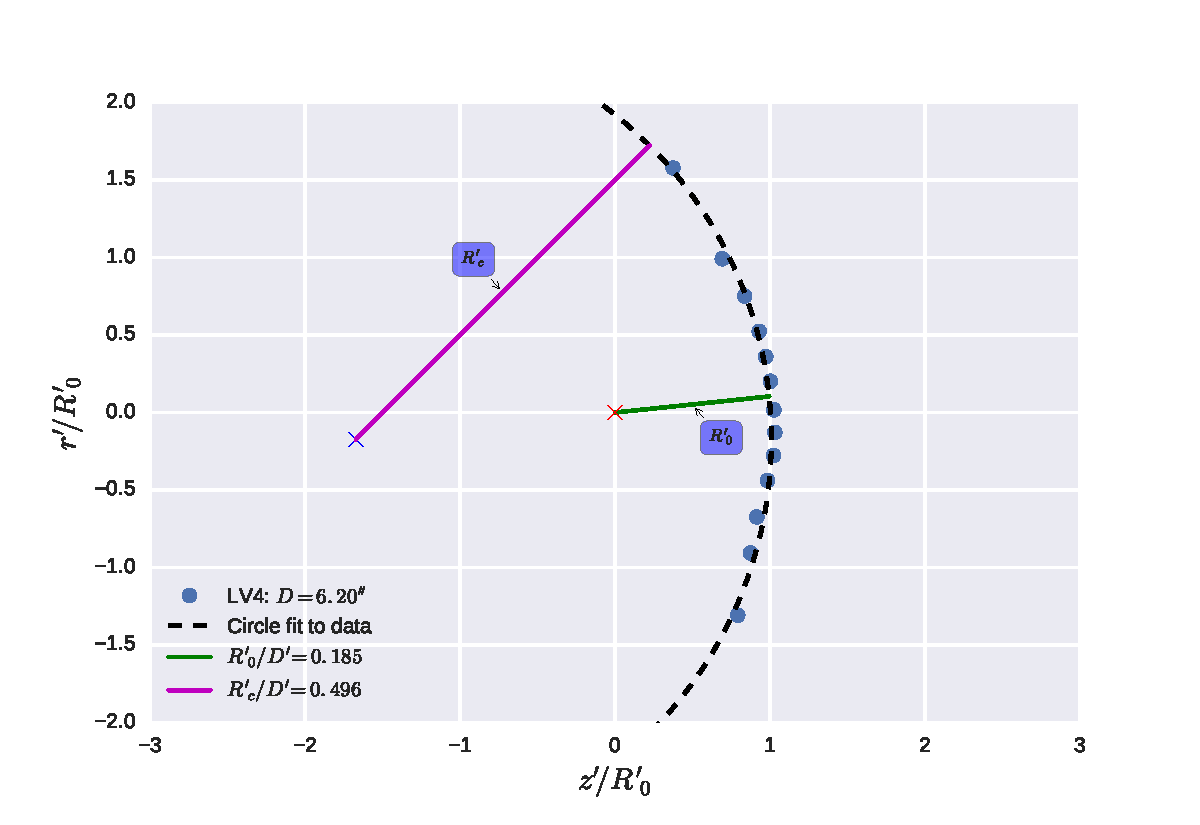
\includegraphics[clip]{./Figures/LV-bowshocks-xyfancy-positionswill-LV4} & 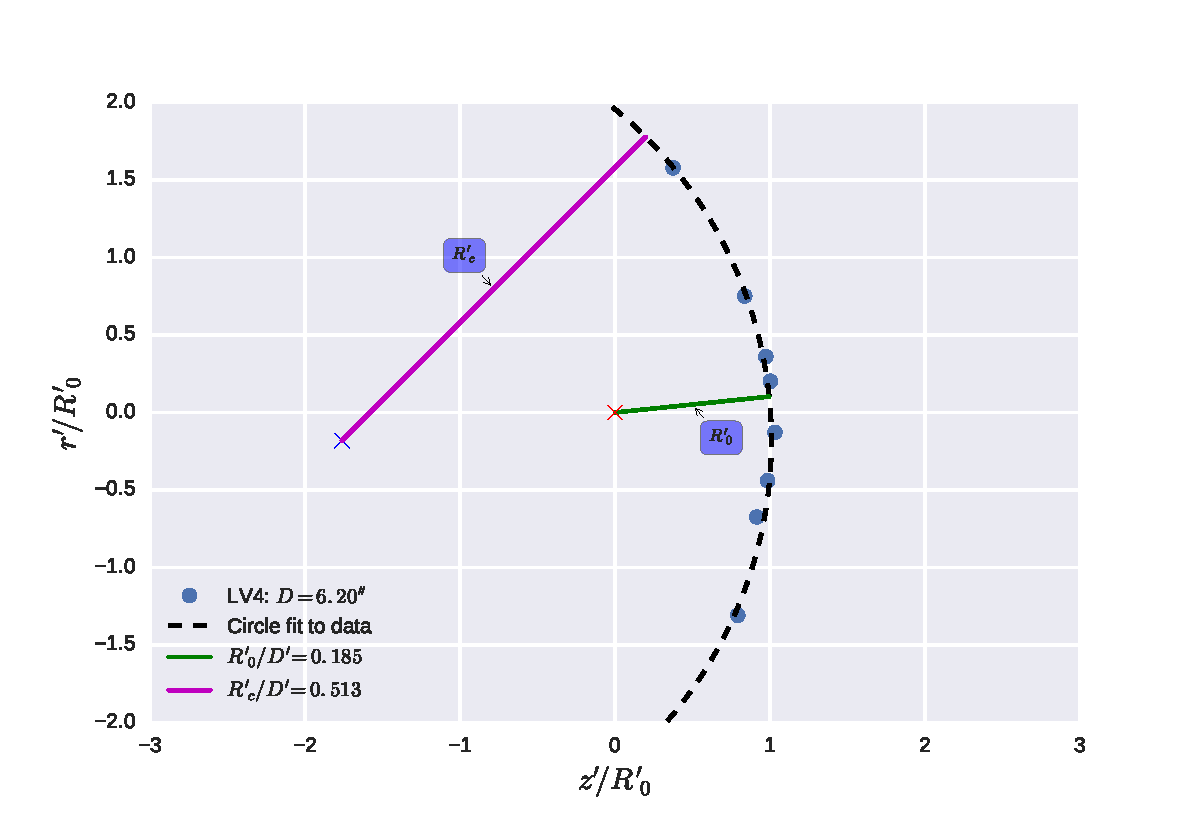
\includegraphics[clip]{./Figures/LV-bowshocks-xyfancy-positionssamp00-LV4} & 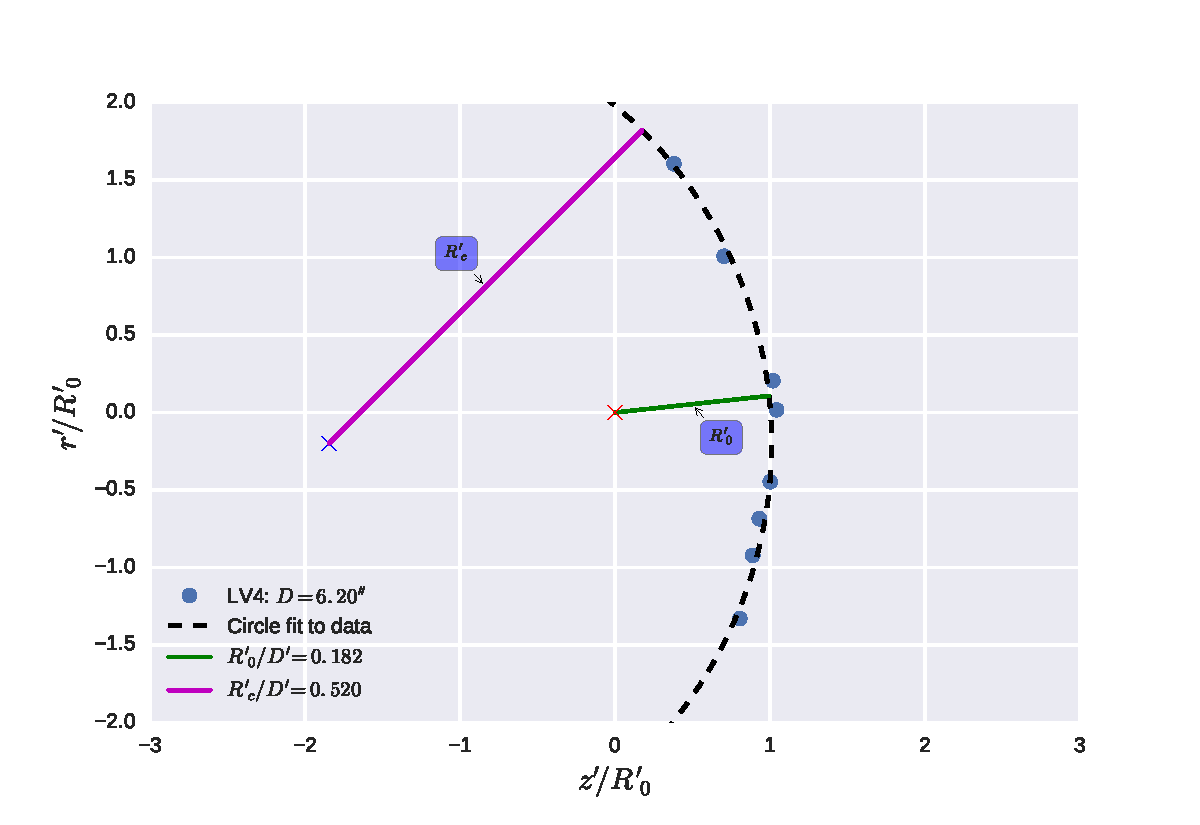
\includegraphics[clip]{./Figures/LV-bowshocks-xyfancy-positionssamp01-LV4} \\
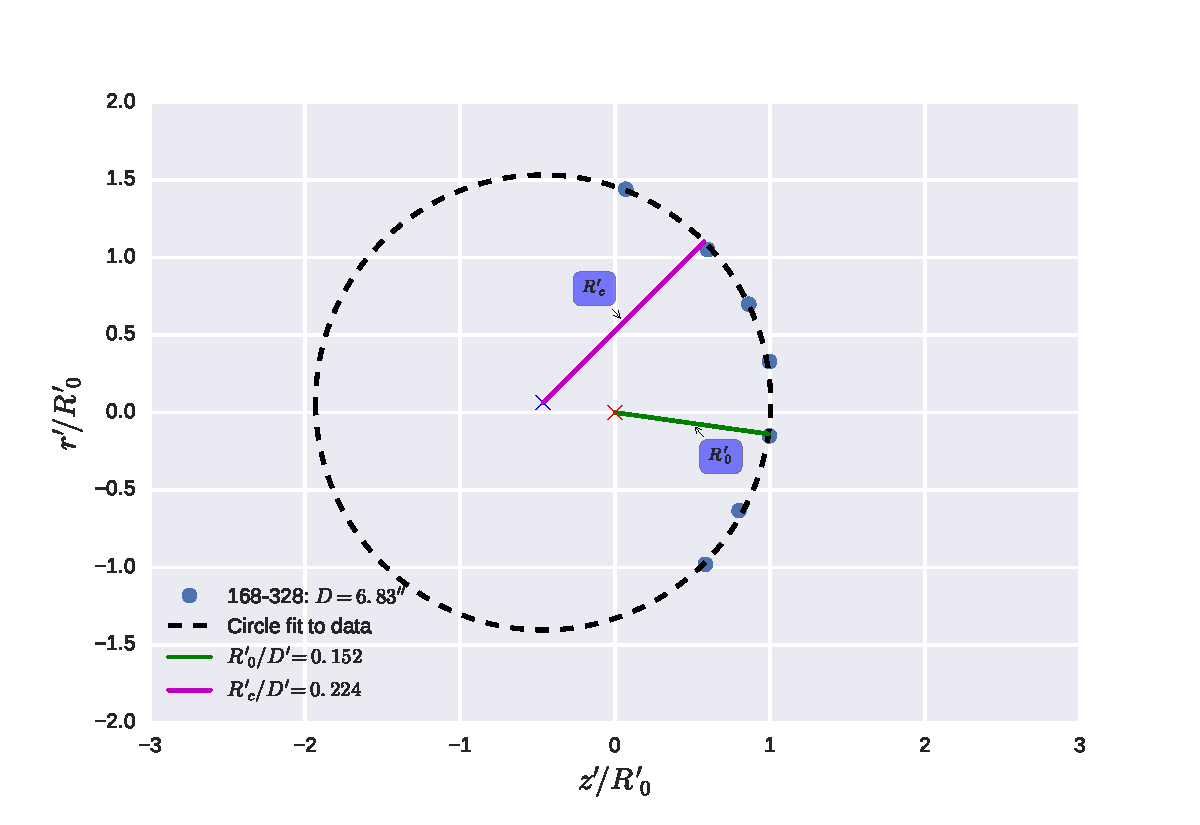
\includegraphics[clip]{./Figures/LV-bowshocks-xyfancy-positionswill-168-328} &  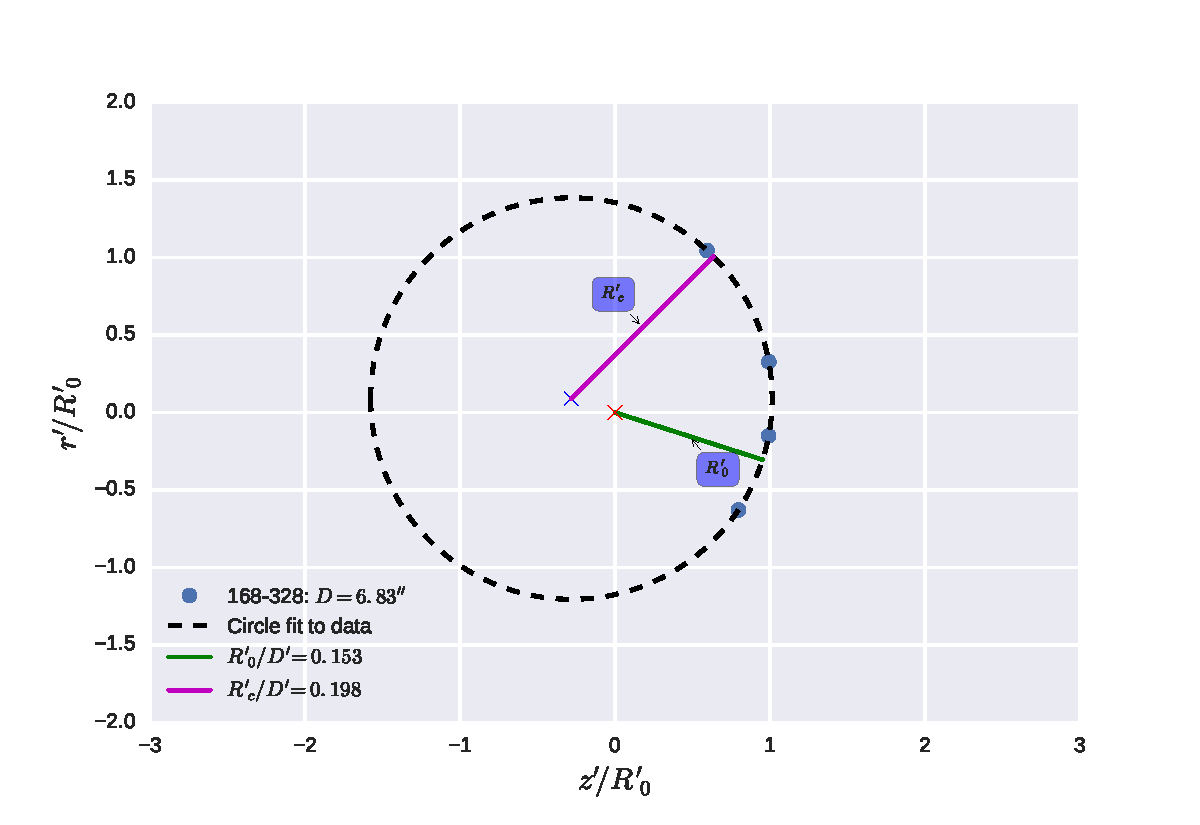
\includegraphics[clip]{./Figures/LV-bowshocks-xyfancy-positionssamp00-168-328} & 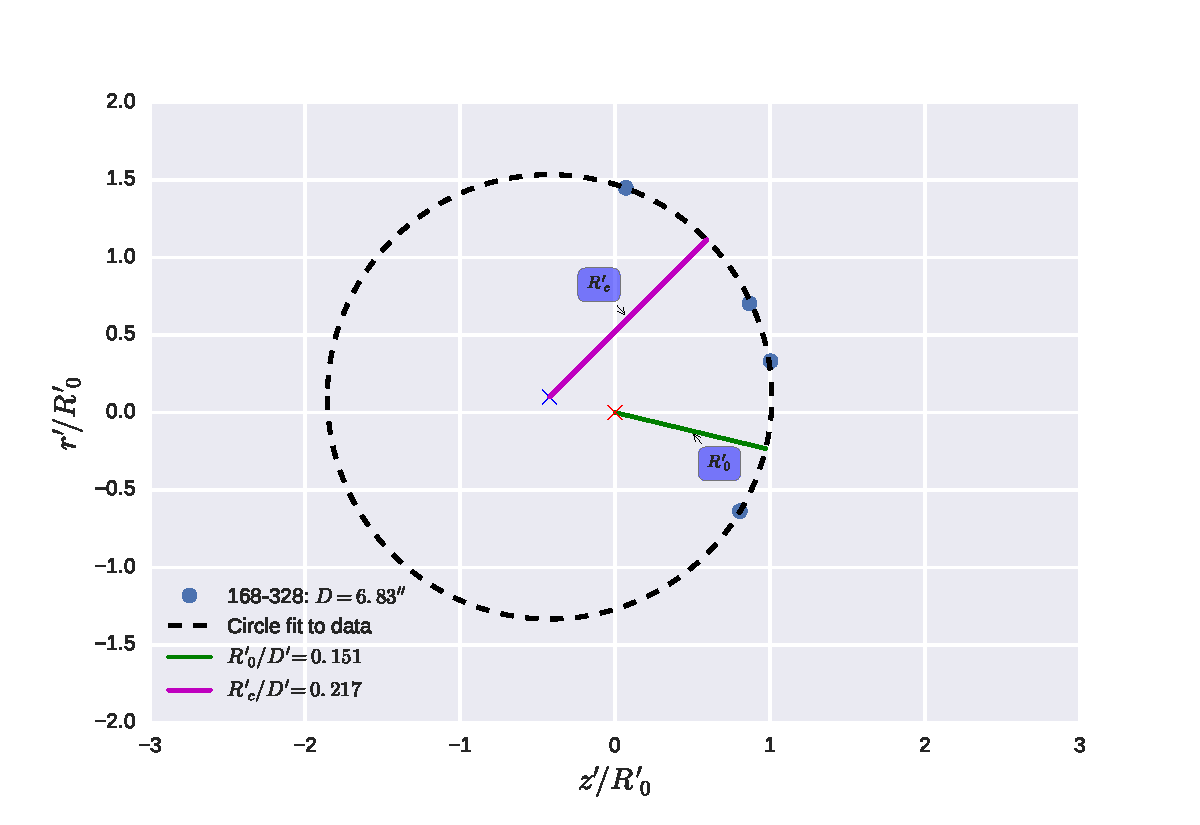
\includegraphics[clip]{./Figures/LV-bowshocks-xyfancy-positionssamp01-168-328}
\end{tabular}
\caption{Ejemplos de incertidumbres sistemáticas en los ajustes circulares a la forma de los choques para tres fuentes (desde la línea superior hasta la inferior): 177-341, LV4 y 168-328. La columna de la izquierda muestra el ajuste a todos los puntos identificados en el borde de la cáscara, donde el número y el espaciamiento de los puntos es una medida subjetiva de nuestra confianza al trazar el borde de cada cáscara. Las dos columnas restantes muestran ajustes a sub-muestras seleccionadas aleatoriamente que contienen 2/3 partes de los puntos de la muestra original para cada cáscara.}
\label{fig:char-radii-obs}
\end{figure*}

\section{Resultados}

Los radios característicos obtenidos para la muestra original y para las submuestras se muestran en la figura \ref{fig:obs-diagnostic}. En cada pánel se utiliza un valor fijo para el parámetro de anisotropía $k$. De esta figura se pueden encontrar algunas observaciones cualitativas: Los proplyds con planitud mayor, LV4 y LV2b ajustan mejor a modelos donde el parámetro de anisotropía es bajo. Para LV2, por otro lado, su medición principal no ajusta a ningún modelo, pero tiene dos variaciones que se desvían mucho de la medición principal que ajustan a modelos con índice de anisotropía alto. Probablemente la presencia de un jet interfiera con la forma del choque (añadir referencia) pero es una hipótesis que va más allá del objetivo de este trabajo. El resto de los proplyds ajusta bien con un parámetro de anisotropía medio $(k\sim 1/2 - 3)$. Dependiendo de los parámetros $(\beta, k)$, la inclinación que se le puede atribuir a cada proplyd en la mayoría de los casos varía entre $15^\circ$ y $40^\circ$  

\begin{figure}
 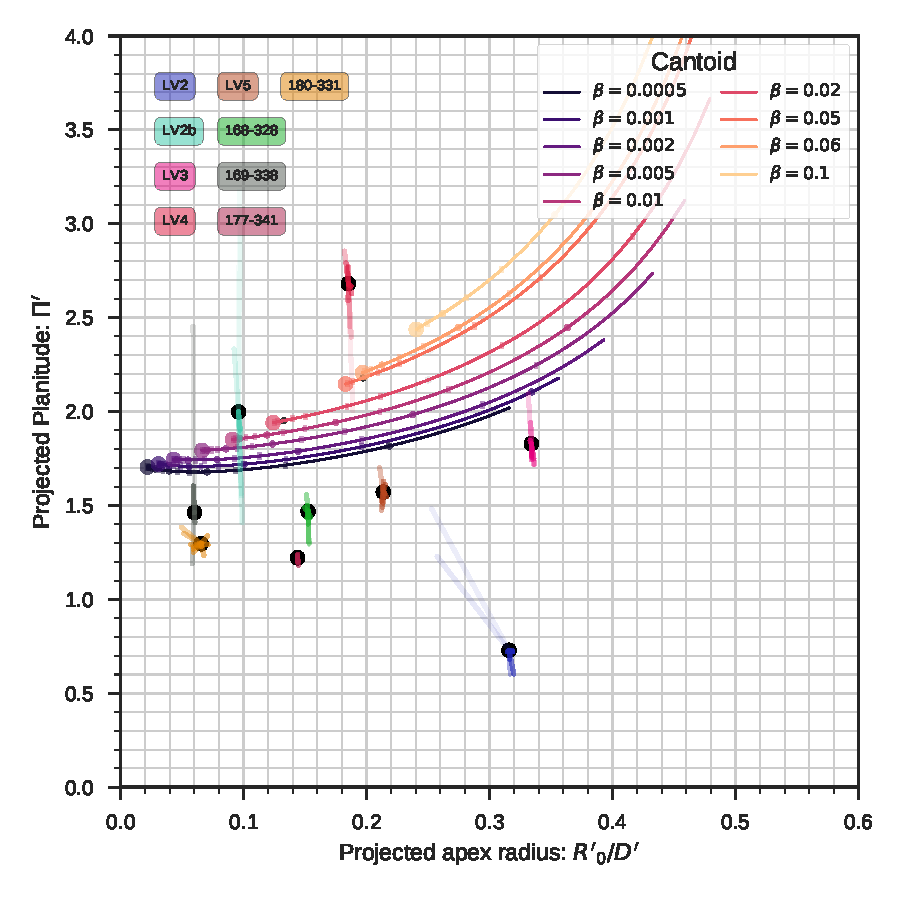
\includegraphics[width=0.48\linewidth]{./Figures/obs-diagnostic-Pi-R0-Cantoid} & 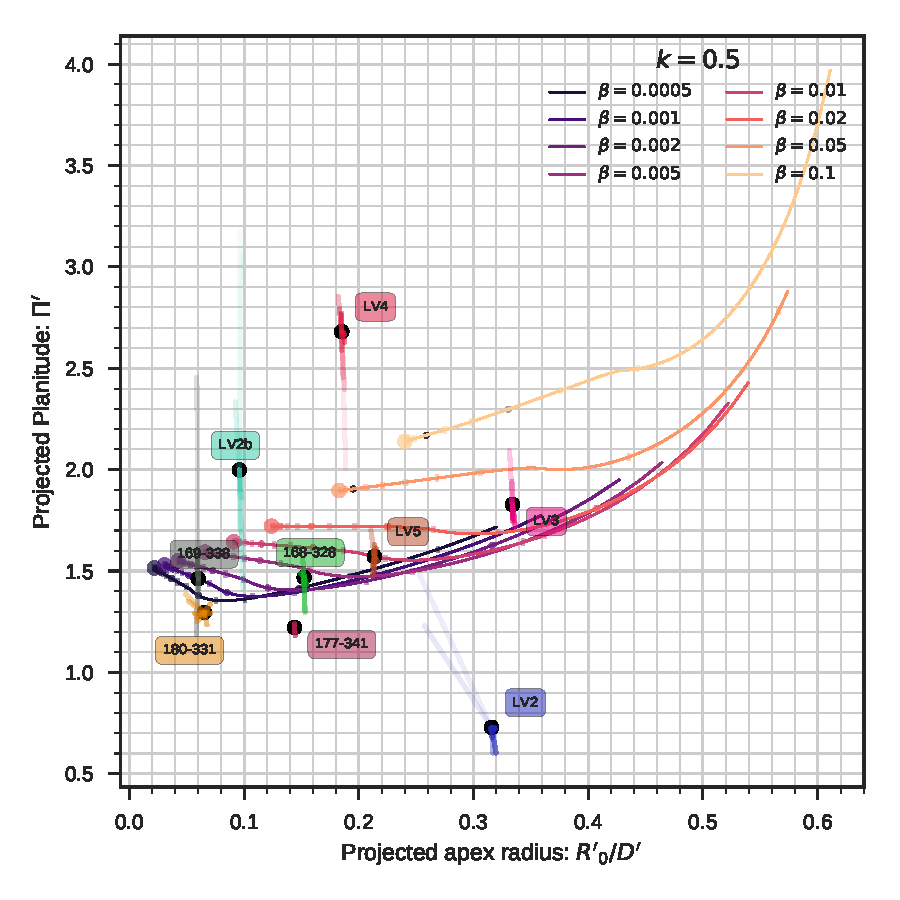
\includegraphics[width=0.48\linewidth]{./Figures/obs-diagnostic-Pi-R0-k05} \\
  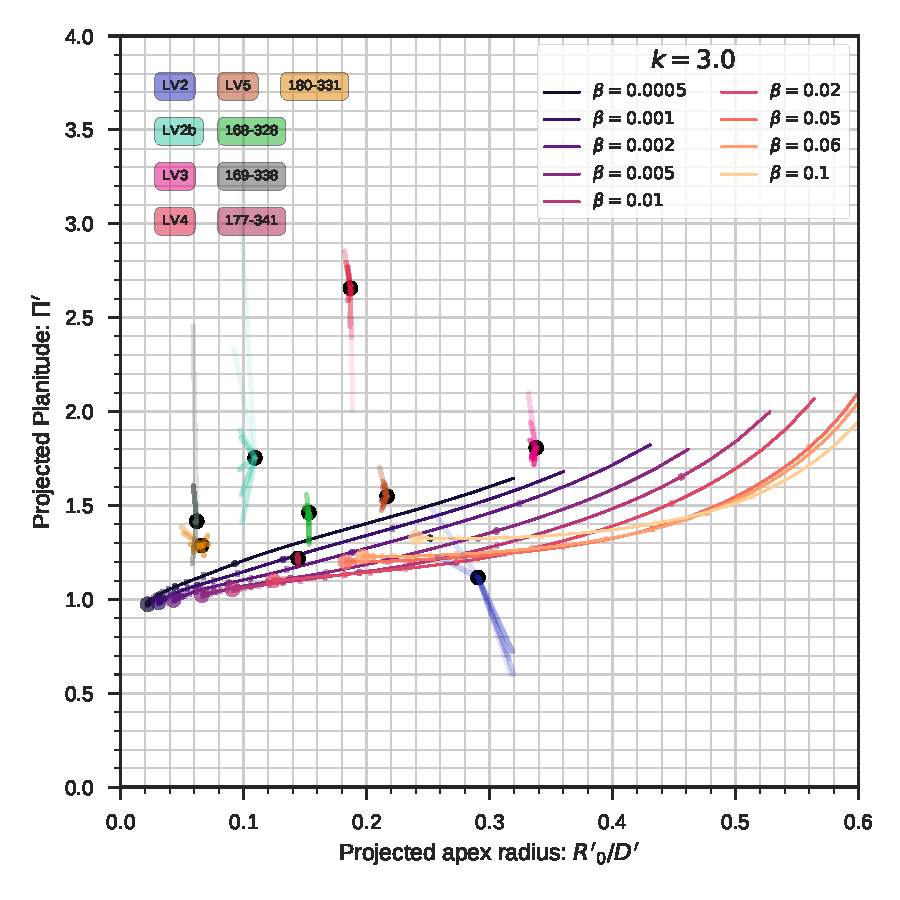
\includegraphics[width=0.48\linewidth]{./Figures/obs-diagnostic-Pi-R0-k30} & 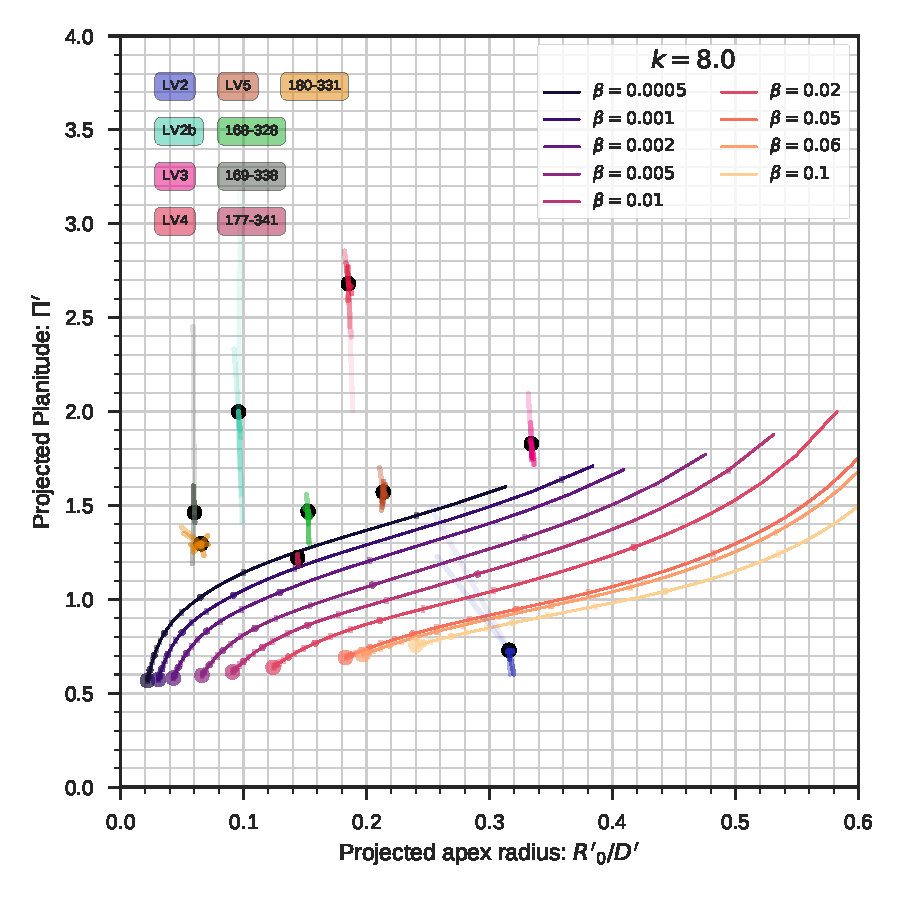
\includegraphics[width=0.48\linewidth]{./Figures/obs-diagnostic-Pi-R0-k80}
  \caption{Similar a la figura \ref{fig:Lambda-Pi-diagram} pero sustituyendo la alatud aparente por el radio aparente en el ápex $R'_0/D'$ para diferentes grados de anisotropía $k$, donde en cada pánel se asume que este parámetro es fijo. A lo largo de cada curva el valor del parámetro $\beta$ es fijo,  mientras que la inclinación se incrementa a lo largo de la curva, empezando a partir del círculo grande, donde $i=0^\circ$. Las marcas circulares pequeñas representan intervalos de $15^\circ$, mientras que las marcas más pequeñas representan intervalos de $5^\circ$. Los resultados observacionales de los choques de proa para nuestro set de proplyds se muestran con puntos negros, mientras que las mediciones de las sub muestras se muestran con líneas de colores radiales que parten desde la medición ``principal''. La opacidad de la medición de cada sub muestra es mayor cuanto menor sea la desviación respecto a la medición principal.}
  \label{fig:obs-diagnostic}
\end{figure}
%\begin{figure*}
%\begin{tabular}{cc}
%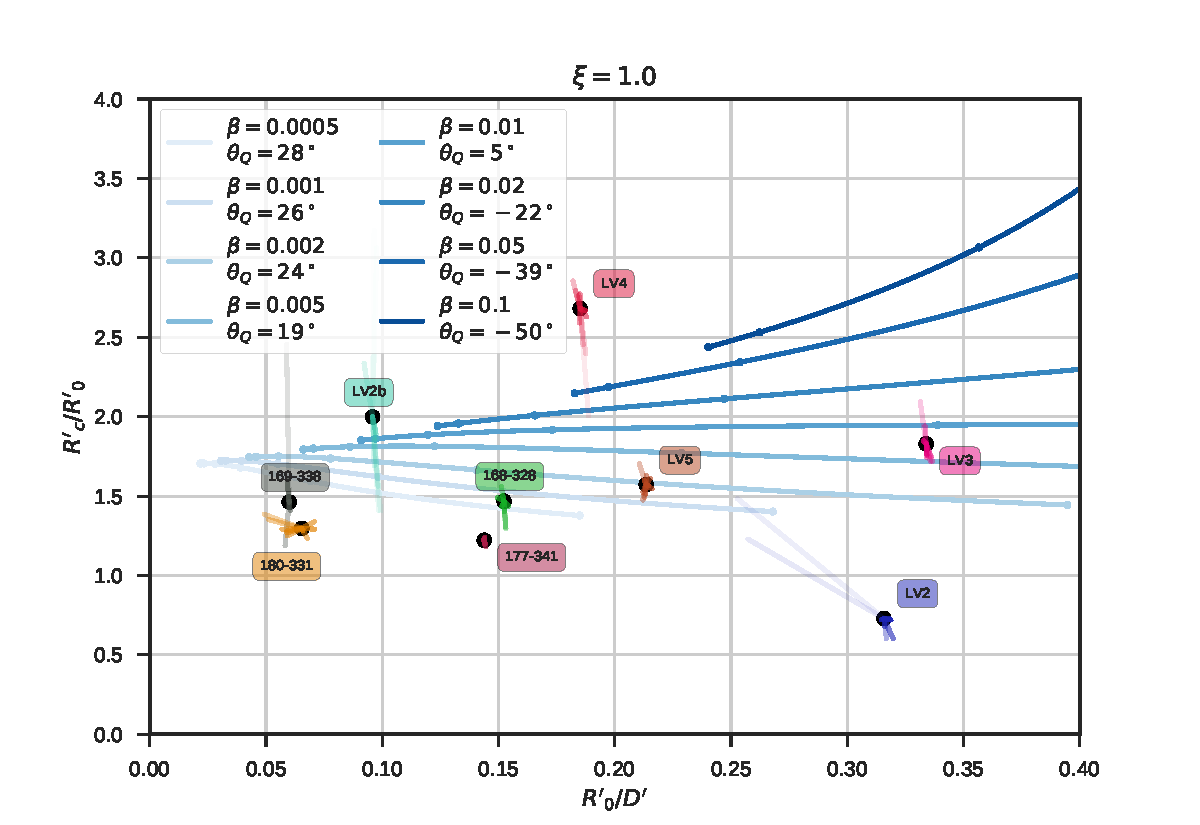
\includegraphics[width=0.48\linewidth]{./Figures/conic_xi-10} & 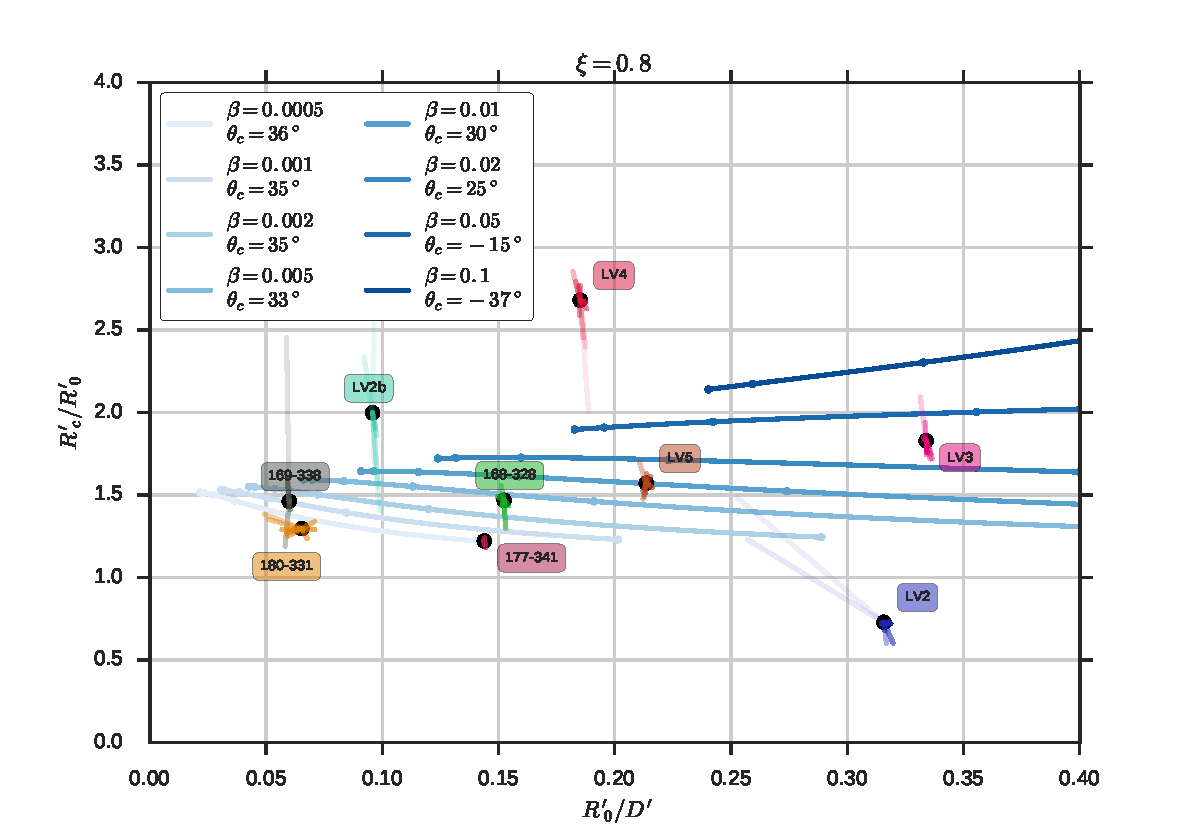
\includegraphics[width=0.48\linewidth]{./Figures/conic_xi-08} \\
%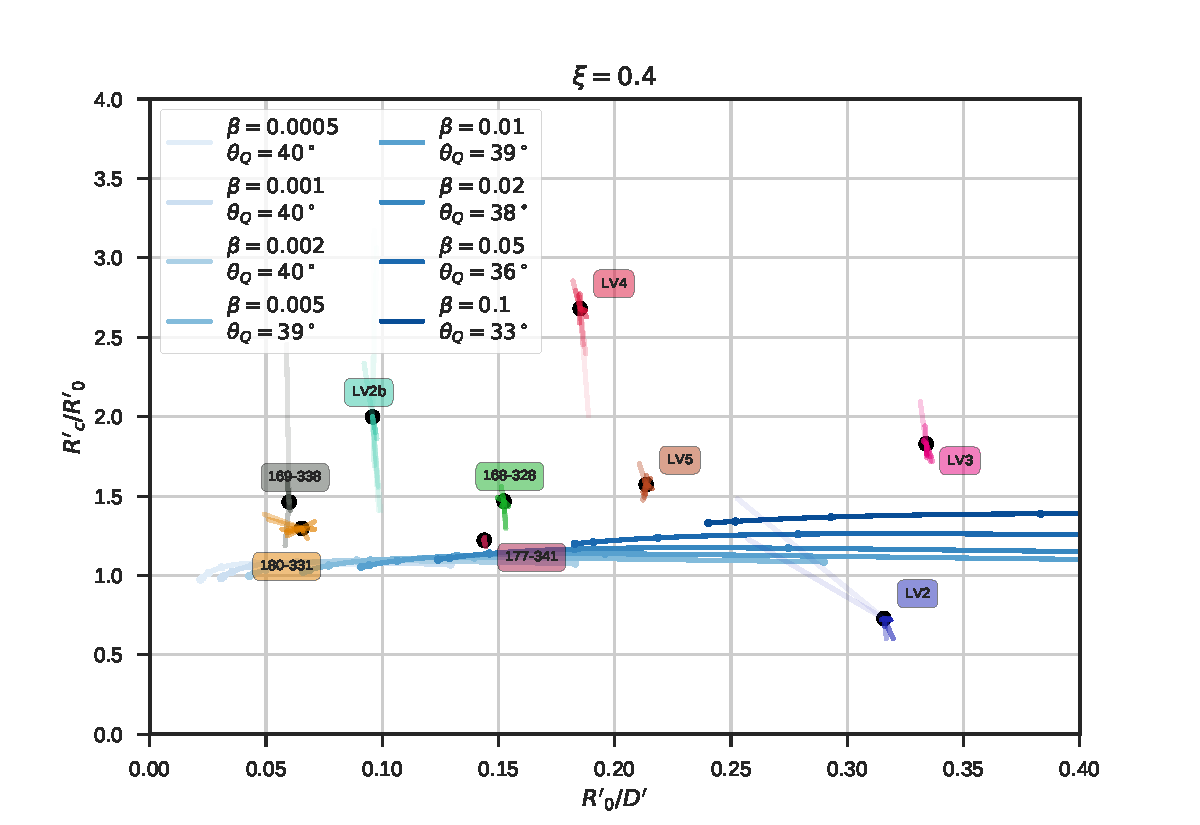
\includegraphics[width=0.48\linewidth]{./Figures/conic_xi-04} & 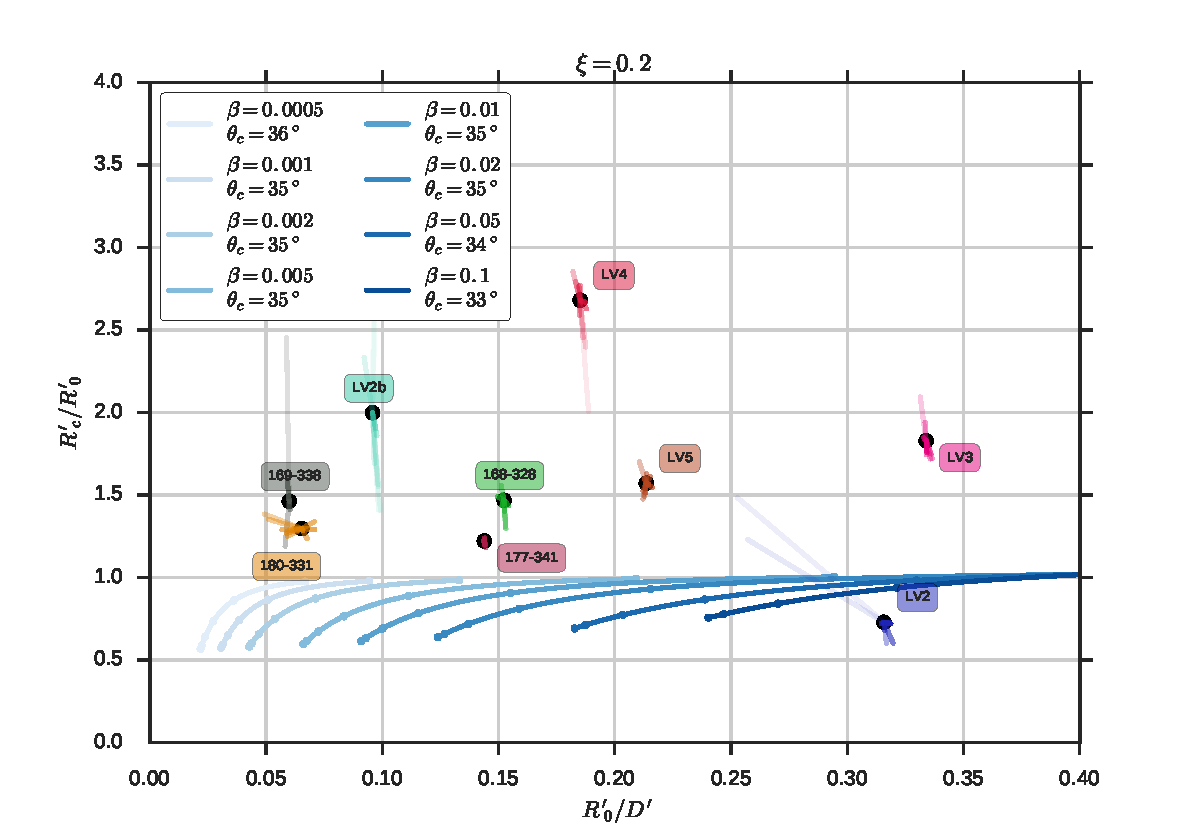
\includegraphics[width=0.48\linewidth]{./Figures/conic_xi-02} 
%\end{tabular}
%\caption{Mediciones de los radios característicos de los proplyds $R_c$ y $R_0$. Las curvas representan el ajuste de una cuádrica para un choque de proa con un cociente de momentos $\beta$ fijo, además se muestra su respectivo valor de $\theta_c$. Los puntos a lo largo de cada curva representan una separación en inclinación de $15^\circ$. Las mediciones para cada proplyd vienen acompañadas con el set de sub-muestras representadas como líneas radiales de colores. En cada gráfica se utiliza un valor diferente para el parámetro de anisotropía $\xi$, iniciando con un viento isotrópico $(\xi=1)$, hasta el viento  con mayor anisotropía $(\xi=0.2)$.}
%\label{fig:conic-xi}
%\end{figure*}

Con base a este análisis, se resume en la tabla \ref{tab:arc-fits} los ajustes a los parámteros de los proplyds: inclinación, distancia a \thC{} intrínseca $D$ y radio del choque en el eje de simetría $R_0/D$.
\begin{landscape}
\begin{table*}
  \caption{Ajuste a los parámetros de los arcos para los choques de proa de los proplyds}
  \label{tab:arc-fits} 
  \newcommand\C[1]{\multicolumn{1}{c}{#1}}
  \begin{adjustbox}{width=1.35\textwidth}
    \small
\begin{tabular}{llrllllrlll}\toprule
             &          & \multicolumn{3}{c}{\dotfill Observado \dotfill}              & \multicolumn{6}{c}{\dotfill Ajuste teórico \dotfill} \\ 
  \C{OW}     & \C{Nombre} & \(D'\) &\C{ \(R_0'/D'\) }&\C{ \(\Pi'_{\mathrm{shape}}\) }&\C{ \(\Pi'_{\mathrm{flux}}\) }&\C{ \(\beta\) }&\C{ \(k\) }&\C{ \(|i|\) }&\C{ \(D\) }&\C{ \(R_0/D\)}\\
  \C{(1)}& \C{ (2) }&\C{ (3)    }&\C{    (4)      }&\C{              (5)           }&\C{           (6)             }&\C{     (7)   }&\C{   (8)   }&\C{   (9) }&\C{  (10) }&\C{   (11)} \\
\midrule     
 168-328  &            &    6.8  &  $0.15 \pm 0.01$  &  $1.45 \pm 0.15$   &  $1.55 \pm 0.05$     &  0.005  &  0.5  &  $52.5 \pm 2.5$   &  $0.022 \pm \SI{1.8e-4}{}$  &  $0.07$  \\
 169-338  &            &  16.4  &  $0.06 \pm 0.01$  &  $1.45^{+1.05}_{-0.25}$   &  $1.65 \pm 0.1$     &  0.002  &  0.0 -- 0.5  &  $35.0 \pm 2.5$   &  $0.040 \pm \SI{1.2e-3}{}$  &  $0.04$  \\
 177-341  & HST1   & 25.6  &  $0.15 \pm 0.01$  &  $1.25 \pm 0.05$   &  $1.25 \pm 0.05$     &  0.0005 -- 0.001  &  3.0 -- 8.0  &  $81.25 \pm 2.8$   &  $0.380 \pm \SI{0.13}{}$  &  $0.03 \pm 0.007$  \\
 180-331  &             &  25.1  &  $0.07^{+0.01}_{-0.03}$  &  $1.3 \pm 0.1$   &  $1.3 \pm 0.1$     &  0.0005  &  0.5  &  $62.5 \pm 2.5$   &  $0.109 \pm \SI{3.6e-4}{}$  &  $0.02$  \\
 167-317  &  LV2     &    7.8  &  $0.31^{+0.01}_{-0.07}$  &  $0.75^{+0.75}_{-0.15}$   &  $1.03 \pm 0.175$      &  0.02 -- 0.1  &  3.0 -- 8.0  &  $42.5 \pm 2.5$  &  $0.021 \pm \SI{9.0e-4}{}$  &  $0.18 \pm 0.06$  \\
 166-316  & LV2b    &   7.2  &  $0.09 \pm 0.01$  &  $2.00^{+1.2}_{-0.6}$   &  $1.78 \pm 0.125$     &  0.01  &  0.0 -- 0.5  &  $16.3 \pm 1.25$  &  $0.015 \pm \SI{1.0e-4}{}$  &  $0.09$  \\
 163-317  & LV3      &   6.9  &  $0.33 \pm 0.01$  &  $1.85^{+0.25}_{0.15}$   &  $2.05 \pm 0.05$     &  0.06  &  0.5  &  $40.0 \pm 2.5$   &  $0.017 \pm \SI{8e-5}{}$  &  $0.2$  \\
 161-324  & LV4      &   6.2  &  $0.19 \pm 0.01$  &  $2.65^{+0.25}_{-0.65}$   &  $2.65^{+0.25}_{-0.65}$     &  0.05  &  0.0  &  $7.5 \pm 2.5$  &  $0.013 \pm \SI{1.2e-5}{}$  &  $0.18$  \\
 168-323  & LV5      &   9.6  &  $0.21 \pm 0.01$  &  $1.55^{+0.15}_{-0.15}$   &  $1.7 \pm 0.05$     &  0.02  &  0.5  &  $42.5 \pm 2.5$   &  $0.026 \pm \SI{1e-4}{}$  &  $0.07$  \\
\bottomrule
\end{tabular}
\end{adjustbox}
\begin{minipage}{0.95\linewidth}
\footnotesize
  Notes --
%
  Col.~(1): ID de la fuente \citep{ODell:1994a}.
%
  Col.~(2): Nombre alternativo de la fuente.
% 
  Col.~(3): Distancia proyectada desde \thC{}, segundos de arco.
%
  Col.~(4): Radio exterior aparente a lo largo del eje, normalizado con la distancia proyectada, donde la incertidumbre es calculada a partir de los valores máximo y mínimo de las submuestras descritas en \S~\ref{sec:methodology}, pero utlizando como mínimo la mitad de la resolución de los ejes de la figura \ref{fig:obs-diagnostic}. Se determina con el ajuste circular decrito en \S~\ref{sec:methodology}.
% 
  Col.~(5): Planitud aparente, donde la incertidumbre es calculada del mismo modo que en Col.~(4). Se determina con el ajuste circular descrito en \S~\ref{sec:methodology}.
% 
  Col.~(6): Planitud aparente, pero aplicando el criterio adicional de que el brillo superficial del proplyd obtenido debe coincidir con la predicción teórica. La medición central corresponde al promedio de las mediciones de las submuestras que cumplen con dicho criterio, con una desviación de $\pm 1\sigma$. Si solo una submuestra cumple el criterio, el resultado de Col.~(5) se traspasa a esta columna. 
%
  Col.~(7): Cociente de momentos entre el viento del proplyd y la estrella O (ver capítulo \ref{chap:hipersonica}). 
% 
  Col.~(8): Parámetro de anisotropía del viento del proplyd.
% 
  Col.~(9): Inclinación respecto al plano del cielo, en grados.
% 
  Col.~(10): Distancia real desde \thC{}, parsecs.
%
  Col.~(11): Radio real de la cáscara a lo largo del eje, normalizado con distancia.

\end{minipage}
\end{table*}
\end{landscape}